\chapter{प्रकाशसंश्लेषण}\label{ch:g12:photosynthesis}

किसी लैंप के नीचे पानी के जार में जलघास की एक टहनी उल्टी रखिए, और उस कटे तने
से बुलबुलों की एक धार उठेगी: ऑक्सीजन, हर कुछ सेकंड पर एक बुलबुला, लैंप पास
लाया जाए तो तेज़, और वह बुझा दिया जाए तो रुक जाती। वह गैस उस प्रक्रिया का
दिखता आधा हिस्सा है जो इस ग्रह के हर जंतु को खिला रही है और जिसने दो अरब साल
पहले हवा साँस लेने लायक़ बनाई। \cref{ch:g10:cell-metabolism} ने उसे एक ही
लकीर में दिया था: कार्बन डाइऑक्साइड और पानी, प्रकाश के साथ, शर्करा तथा
ऑक्सीजन बन जाते हैं। यह अध्याय \omterm{def:g12:photosynthesis:chloroplast}{हरितलवक} खोलता है और किसी फ़ोटॉन की ऊर्जा के
पीछे-पीछे किसी रासायनिक बंध तक जाता है।

\section{वह हरितलवक}

\begin{definition}[हरितलवक]\label{def:g12:photosynthesis:chloroplast}
\emph{हरितलवक}\index{हरितलवक} \omterm{def:g10:cell-metabolism:autotrophy}{प्रकाशसंश्लेषण} का \omterm{def:g10:cells-common-unit:organelle}{कोशिकांग} है: कोई
\qty{5}{\micro m} लंबी लेंस जैसी काया, जो दोहरी झिल्ली से घिरी है और जिसमें
एक तरल, यानी \emph{पीठिका}, है, तथा उसमें चपटी झिल्ली थैलियों के चट्टे, यानी
\emph{थाइलेकॉइड}\index{थाइलेकॉइड}, पड़े हैं। थाइलेकॉइड झिल्लियाँ वर्णक
थामती हैं --- \emph{पर्णहरित} a तथा b, जो हरे हैं, और नारंगी कैरोटिनॉइड ---
और वे \omterm{def:g11:gene-expression:protein}{प्रोटीन} भी जो प्रकाश ऊर्जा बदलते हैं; जबकि वह पीठिका उन एंजाइमों को
थामती है जो शर्करा बनाते हैं। किसी पत्ती \omterm{def:g10:cells-common-unit:cell}{कोशिका} में दर्जनों हरितलवक होते
हैं, और पत्ते के एक वर्ग मिलीमीटर में कोई पाँच लाख।
\end{definition}

\begin{omfigure}
\begin{tikzpicture}
  \node[anchor=south west, inner sep=0] (img) at (0,0)
    {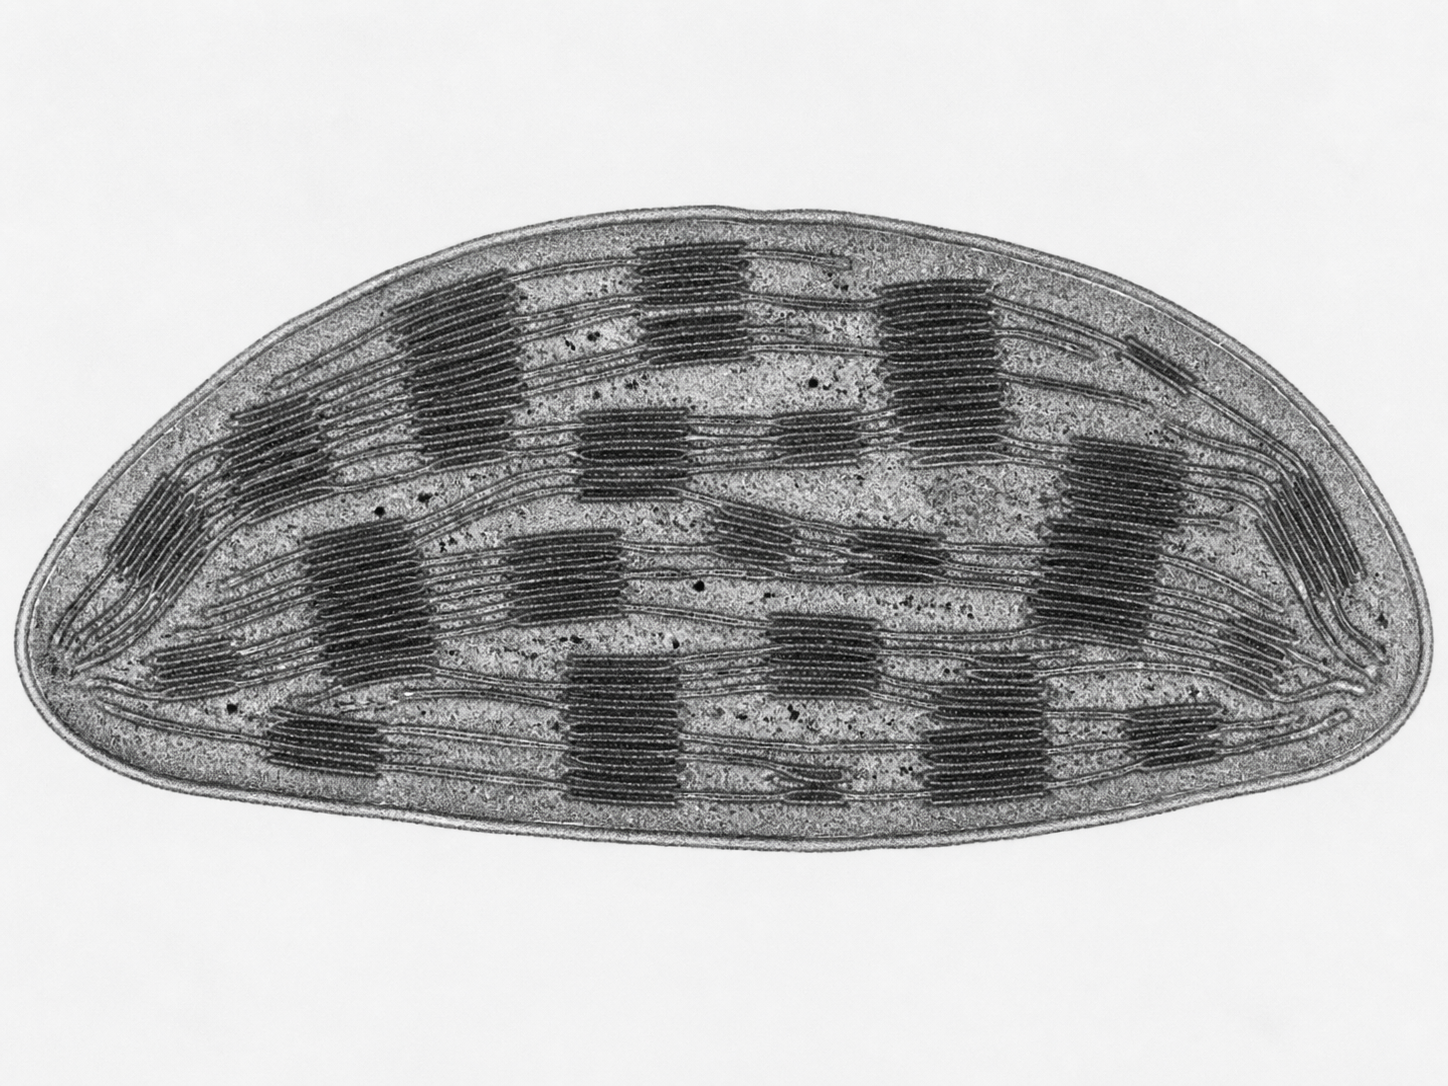
\includegraphics[width=0.5\linewidth]{images/book2/ai/g12-photo-chloroplast-tem.png}};
  \begin{scope}[x={(img.south east)}, y={(img.north west)},
      every node/.style={font=\small}]
    \draw[omDef, thick] (0.10,0.50) -- (-0.04,0.80) node[left, align=right] {दोहरा\\ आवरण};
    \draw[omDef, thick] (0.47,0.72) -- (0.47,1.06) node[above] {चट्टे बने थाइलेकॉइड (एक ग्रैनम)};
    \draw[omDef, thick] (0.62,0.42) -- (1.04,0.20) node[right] {पीठिका};
    \draw[omDef, thick] (0.80,0.60) -- (1.04,0.75) node[right, align=left] {चट्टों को जोड़ती\\ झिल्लियाँ};
  \end{scope}
\end{tikzpicture}

{\small इलेक्ट्रॉन सूक्ष्मदर्शी में एक \omterm{def:g12:photosynthesis:chloroplast}{हरितलवक}: वह दोहरा आवरण, वह पीठिका,
और ग्रैनमों में चट्टे बनी \omterm{def:g12:photosynthesis:chloroplast}{थाइलेकॉइड} झिल्लियाँ, जहाँ वर्णक बैठते हैं।
प्रकाश उन झिल्लियों में पकड़ा जाता है; और शर्करा उनके चारों ओर के तरल में
बनाई जाती है।}
\end{omfigure}

\begin{proposition}[कौन-सा प्रकाश इस्तेमाल होता है]\label{prop:g12:photosynthesis:spectrum}
पर्णहरित नीला तथा लाल प्रकाश ज़ोर से अवशोषित करता है और हरा प्रकाश शायद ही
--- इसीलिए पत्ते हरे हैं। \omterm{def:g10:cell-metabolism:autotrophy}{प्रकाशसंश्लेषण} उन्हीं तरंगदैर्घ्यों से चलता है जो
वे वर्णक अवशोषित करते हैं: तरंगदैर्घ्य के सामने नापने पर उसकी दर (यानी
\emph{क्रिया स्पेक्ट्रम}) उन वर्णकों के अवशोषण के साथ चढ़ती-उतरती है, जिसकी
चोटियाँ नीले तथा लाल में और गड्ढा हरे में है।
\end{proposition}
\begin{proof}[साक्ष्य]
एंगेलमान (1882) ने किसी हरे शैवाल का एक तंतु पानी की ऐसी बूँद में रखा जिसमें
ऐसे जीवाणु थे जो ऑक्सीजन की ओर तैरते हैं, और सूक्ष्मदर्शी से उस तंतु पर एक
स्पेक्ट्रम डाला: वे जीवाणु नीले तथा लाल में रोशन हिस्सों के इर्द-गिर्द जमा
हो गए, और हरे से दूर रहे --- यानी ऑक्सीजन वहीं छोड़ी जा रही थी जहाँ वे रंग
पड़े। रंगीन लैंपों के नीचे ऑक्सीजन उत्पादन का आधुनिक मापन वही वक्र देता है,
और वह निकाले गए वर्णकों के अवशोषण स्पेक्ट्रम से मेल खाता है।
\end{proof}

\begin{omfigure}
\begin{tikzpicture}
\begin{axis}[
  width=0.88\linewidth, height=5.8cm,
  axis x line=bottom, axis y line=left,
  xmin=400, xmax=700, ymin=0, ymax=110,
  xlabel={तरंगदैर्घ्य (nm)}, ylabel={अधिकतम का \%},
  xlabel style={font=\small, at={(axis description cs:0.5,-0.12)}, anchor=north},
  ylabel style={font=\small},
  tick label style={font=\small}, xtick={400,450,500,550,600,650,700}, ytick={0,50,100},
  legend style={at={(0.5,-0.3)}, anchor=north, legend columns=2, font=\small, draw=none},
]
\addplot[thick, omMeth, smooth] coordinates {(400,70) (430,100) (450,75) (480,35) (500,15) (550,8) (600,15) (640,45) (665,90) (680,70) (700,10)};
\addplot[thick, omThm, dashed, smooth] coordinates {(400,65) (430,85) (450,80) (480,55) (500,35) (550,25) (600,35) (640,60) (665,95) (680,100) (700,20)};
\legend{पत्ती वर्णकों द्वारा अवशोषण, प्रकाशसंश्लेषण की दर (क्रिया स्पेक्ट्रम)}
\end{axis}
\end{tikzpicture}

{\small किसी पत्ते के निकाले गए वर्णकों द्वारा प्रकाश का अवशोषण, और उस
पत्ते के \omterm{def:g10:cell-metabolism:autotrophy}{प्रकाशसंश्लेषण} की दर, तरंगदैर्घ्य के सामने। दोनों नीले तथा लाल में
चोटी छूते हैं और हरे में बैठ जाते हैं: यानी जो प्रकाश \omterm{def:g10:cell-metabolism:autotrophy}{प्रकाशसंश्लेषण} चलाता
है वही प्रकाश है जो वे वर्णक अवशोषित करते हैं।}
\end{omfigure}

\section{प्रकाश प्रावस्था: पानी चिरा, ऊर्जा जमा}

\begin{proposition}[थाइलेकॉइडों में क्या होता है]\label{prop:g12:photosynthesis:lightphase}
\omterm{def:g12:photosynthesis:chloroplast}{थाइलेकॉइड} झिल्लियों में, प्रकाश में, तीन चीज़ें एक साथ होती हैं:
\begin{itemize}
  \item पानी के अणु \emph{चीरे} जाते हैं: उनकी ऑक्सीजन $\mathrm{O_2}$ की
        तरह छोड़ दी जाती है --- यानी \omterm{def:g10:cell-metabolism:autotrophy}{प्रकाशसंश्लेषण} की ऑक्सीजन पानी से आती
        है, कार्बन डाइऑक्साइड से नहीं --- और उनका हाइड्रोजन इलेक्ट्रॉनों
        तथा प्रोटॉनों की तरह रोक लिया जाता है;
  \item अवशोषित फ़ोटॉनों की ऊर्जा उन इलेक्ट्रॉनों को किसी वाहक अणु, यानी
        \emph{अपचयित NADP}, पर लादने में इस्तेमाल होती है, जिसे वह पीठिका
        हाइड्रोजन के स्रोत की तरह इस्तेमाल करेगी;
  \item वही ऊर्जा \emph{ATP} का संश्लेषण चलाती है।
\end{itemize}
इस तरह प्रकाश प्रावस्था प्रकाश को दो रासायनिक उत्पादों में बदल देती है, यानी
ATP तथा अपचयित NADP, और उपोत्पाद की तरह ऑक्सीजन छोड़ती है। इसमें कोई कार्बन
डाइऑक्साइड शामिल नहीं है।
\end{proposition}
\begin{proof}[साक्ष्य]
हिल (1937) ने अलग किए \omterm{def:g12:photosynthesis:chloroplast}{हरितलवक} पानी में किसी बनावटी इलेक्ट्रॉन ग्राही के साथ
और बिना किसी कार्बन डाइऑक्साइड के रोशन किए: उन्होंने ऑक्सीजन छोड़ी और उस
ग्राही को अपचयित किया। यानी ऑक्सीजन के छोड़े जाने को प्रकाश तथा पानी चाहिए
पर $\mathrm{CO_2}$ नहीं, और वह इलेक्ट्रॉनों के अंतरण से जुड़ा है। रूबेन और
कामेन (1941) ने शैवालों को ऐसा पानी दिया जिसमें भारी समस्थानिक $^{18}$O था:
छोड़ी गई ऑक्सीजन भारी थी; और भारी कार्बन डाइऑक्साइड तथा साधारण पानी देने
पर वह भारी नहीं थी। वह ऑक्सीजन पानी से आती है।
\end{proof}

\begin{omfigure}
\begin{tikzpicture}[font=\small, >=Stealth,
  b/.style={draw, rounded corners, align=center, minimum height=1.0cm}]
  % thylakoid box
  \node[b, fill=omMeth!15, text width=3.6cm, minimum height=3.2cm] (thy) at (0,0) {};
  \node[anchor=north, font=\small\bfseries] at (thy.north) {थाइलेकॉइड झिल्लियाँ};
  \node[font=\small, align=center] at (0,-0.1) {पर्णहरित द्वारा\\ अवशोषित प्रकाश};
  % stroma box
  \node[b, fill=omDef!10, text width=3.6cm, minimum height=3.2cm] (str) at (6.4,0) {};
  \node[anchor=north, font=\small\bfseries] at (str.north) {पीठिका};
  \node[font=\small, align=center] at (6.4,-0.1) {कैल्विन चक्र:\\ $\mathrm{CO_2}$ शर्करा\\ में बाँधी गई};
  % inputs/outputs
  \draw[->, thick, omProp] (-3.2,1.0) -- (thy.west |- 0,1.0) node[pos=0, left, omProp] {प्रकाश};
  \draw[->, thick] (-3.2,-0.6) -- (thy.west |- 0,-0.6) node[pos=0, left] {$\mathrm{H_2O}$};
  \draw[->, thick] (thy.south) -- ++(0,-1.0) node[below] {$\mathrm{O_2}$ छोड़ी गई};
  \draw[->, thick, omThm] (thy.east |- 0,0.7) -- (str.west |- 0,0.7) node[midway, above] {ATP};
  \draw[->, thick, omThm] (thy.east |- 0,-0.3) -- (str.west |- 0,-0.3) node[midway, above] {अपचयित NADP};
  \draw[->, thick, gray] (str.west |- 0,-1.1) -- (thy.east |- 0,-1.1) node[midway, below, font=\scriptsize] {वाहक लौटते हैं};
  \draw[->, thick] (9.6,0.6) -- (str.east |- 0,0.6) node[pos=0, right] {$\mathrm{CO_2}$};
  \draw[->, thick] (str.east |- 0,-0.6) -- (9.6,-0.6) node[right] {शर्करा};
\end{tikzpicture}

{\small \omterm{def:g10:cell-metabolism:autotrophy}{प्रकाशसंश्लेषण} की दोनों प्रावस्थाएँ। \omterm{def:g12:photosynthesis:chloroplast}{थाइलेकॉइड} झिल्लियों में प्रकाश
पानी चीरता है, ऑक्सीजन छोड़ता है और दो वाहक, यानी ATP तथा अपचयित NADP, चार्ज
करता है। और पीठिका में वे वाहक कार्बन डाइऑक्साइड को शर्करा में बाँधने की
क़ीमत चुकाते हैं। पहली प्रावस्था को प्रकाश चाहिए; और दूसरी को केवल उसके
उत्पाद।}
\end{omfigure}

\section{कार्बन प्रावस्था: शर्करा बनी}

\begin{proposition}[कैल्विन चक्र]\label{prop:g12:photosynthesis:calvin}
पीठिका में कार्बन डाइऑक्साइड, एक बार में एक अणु, पहले से मौजूद किसी
पाँच-कार्बन शर्करा से पृथ्वी के सबसे प्रचुर \omterm{def:g11:enzymes-and-phenotype:enzyme}{एंजाइम} द्वारा जोड़ दी जाती है;
और छह-कार्बन वाला उत्पाद तुरंत दो तीन-कार्बन अणुओं में चिर जाता है, जो
प्रकाश प्रावस्था के ATP तथा अपचयित NADP से अपचयित होकर तीन-कार्बन शर्कराएँ
बनते हैं। इनमें से अधिकांश उस पाँच-कार्बन ग्राही को दोबारा बनाने में
पुनर्चक्रित होती हैं, जिससे \emph{कैल्विन चक्र}\index{कैल्विन चक्र} बंद हो
जाता है; और छह में से एक उस चक्र से उस पौधे के शुद्ध लाभ की तरह निकलती है।
चक्र के तीन फेरे, तीन $\mathrm{CO_2}$ बँधीं, नौ ATP तथा छह अपचयित NADP
ख़र्च: और एक तीन-कार्बन शर्करा बाहर भेजी गई। उनमें से दो एक ग्लूकोज बनाती
हैं।
\end{proposition}
\begin{proof}[साक्ष्य]
कैल्विन (1950 के दशक में) ने शैवालों को कुछ ही सेकंड के लिए रेडियोसक्रिय
$^{14}$C से चिह्नित कार्बन डाइऑक्साइड दी, उन्हें खौलती एल्कोहल में मार
डाला, और उनके अणु अलग किए: पाँच सेकंड बाद वह चिह्न किसी एक तीन-कार्बन अम्ल
में था; तीस बाद, तीन-कार्बन शर्कराओं तथा उस पाँच-कार्बन ग्राही में; और कुछ
मिनट बाद, सुक्रोज तथा मंड में। प्रकाश काट देने पर वह ग्राही दोबारा बनना बंद
हो गया और वह तीन-कार्बन अम्ल जमा होने लगा; और $\mathrm{CO_2}$ काट देने पर
वह ग्राही जमा होने लगा। प्रकट होने का क्रम ही उस चक्र का क्रम है।
\end{proof}

\begin{omfigure}
\begin{tikzpicture}[font=\small, >=Stealth]
  \draw[thick, ->] (90:2.2) arc (90:-30:2.2);
  \draw[thick, ->] (-30:2.2) arc (-30:-150:2.2);
  \draw[thick, ->] (-150:2.2) arc (-150:-270:2.2);
  \node[draw, rounded corners, fill=omDef!12, align=center, font=\small] at (90:2.2) {5-कार्बन\\ ग्राही ($\times 3$)};
  \node[draw, rounded corners, fill=omProp!15, align=center, font=\small] at (-30:2.2) {3-कार्बन अम्ल\\ ($\times 6$)};
  \node[draw, rounded corners, fill=omMeth!15, align=center, font=\small] at (-150:2.2) {3-कार्बन शर्करा\\ ($\times 6$)};
  \draw[->, thick] (3.6,2.2) -- (2.4,1.6) node[pos=0, right, align=left] {$3\,\mathrm{CO_2}$ घुसती हैं};
  \draw[->, thick, omThm] (2.2,-2.4) -- (1.2,-2.0) node[pos=0, right, omThm, align=left] {प्रकाश प्रावस्था से\\ 6 ATP, 6 अपचयित NADP};
  \draw[->, thick, omThm] (-3.6,1.0) -- (-2.2,1.4) node[pos=0, left, omThm] {3 ATP};
  \draw[->, thick] (-2.4,-2.4) -- (-3.6,-3.2) node[anchor=north, align=center] {1 तीन-कार्बन शर्करा निकलती है:\\ आधा ग्लूकोज};
  \node[font=\scriptsize, align=center] at (0,0) {6 में से 5 शर्कराएँ\\ 3 ग्राही दोबारा\\ बनाती हैं};
\end{tikzpicture}

{\small \omterm{prop:g12:photosynthesis:calvin}{कैल्विन चक्र}, तीन फेरों के लिए गिना गया। तीन कार्बन डाइऑक्साइड तीन
पाँच-कार्बन ग्राहियों से जुड़ती हैं; छहों तीन-कार्बन उत्पाद प्रकाश
प्रावस्था के ATP तथा अपचयित NADP की क़ीमत पर शर्कराओं में अपचयित होते हैं;
और छह में से पाँच ग्राहियों में पुनर्चक्रित हो जाती हैं तथा एक ही लाभ है।}
\end{omfigure}

\begin{example}[किसी ग्लूकोज का बहीखाता]\label{ex:g12:photosynthesis:bookkeeping}
एक ग्लूकोज को छह कार्बन डाइऑक्साइड चाहिए, यानी उस चक्र के छह फेरे, 18 ATP
तथा 12 अपचयित NADP, जो सब प्रकाश प्रावस्था जुटाती है, जो उन्हें बनाने के लिए
12 पानी के अणु चीरती है और छह ऑक्सीजन छोड़ती है। शुद्ध:
$6\,\mathrm{CO_2} + 12\,\mathrm{H_2O} \to \mathrm{C_6H_{12}O_6} +
6\,\mathrm{O_2} + 6\,\mathrm{H_2O}$ --- यानी
\cref{ch:g10:cell-metabolism} वाला सारांश समीकरण, अब दोनों ओर पानी के साथ,
क्योंकि छोड़ी गई ऑक्सीजन चीरे गए पानी से आती है, कार्बन डाइऑक्साइड से नहीं।
\end{example}

\begin{omfigure}
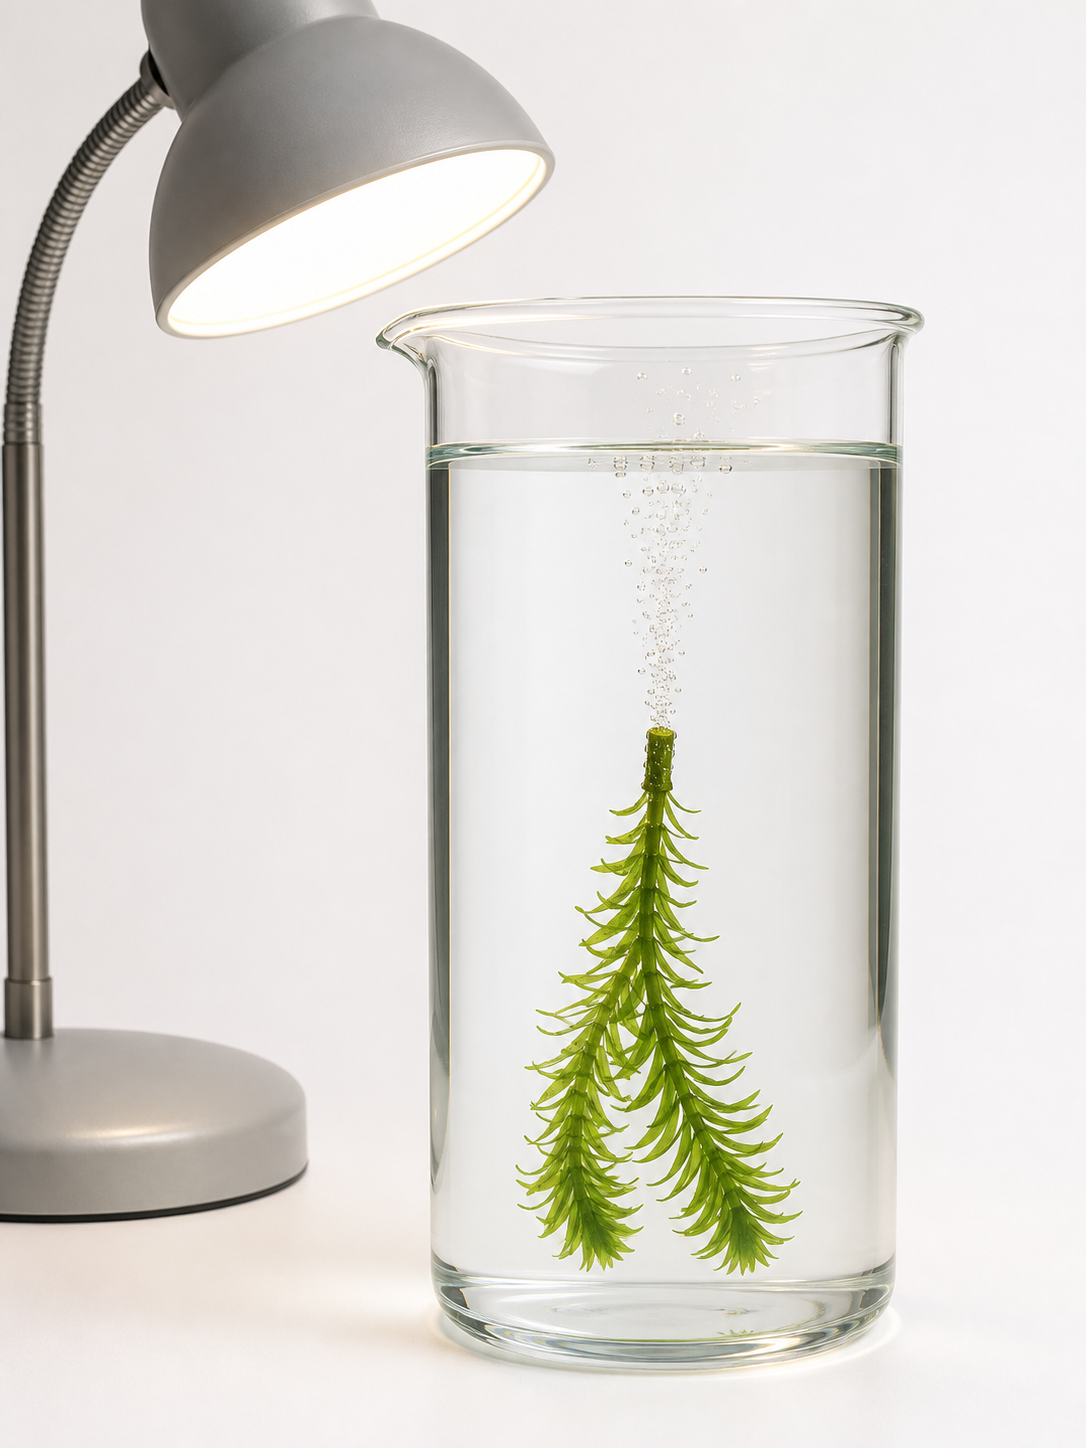
\includegraphics[width=0.34\linewidth]{images/book2/ai/g12-photo-elodea-bubbles.png}

{\small किसी लैंप के नीचे जलघास: उस कटे तने से उठते बुलबुले प्रकाश प्रावस्था
की ऑक्सीजन हैं। उन्हें प्रति मिनट गिनिए, लैंप हिलाइए, उसका रंग बदलिए, और
\omterm{def:g10:cell-metabolism:autotrophy}{प्रकाशसंश्लेषण} की दर नप जाती है।}
\end{omfigure}

\section{वह शर्करा क्या बनती है, और कितनी है}

\begin{proposition}[उस उत्पाद की क़िस्मतें]\label{prop:g12:photosynthesis:fates}
उस चक्र से निकलती तीन-कार्बन शर्कराएँ \omterm{def:g12:photosynthesis:chloroplast}{हरितलवक} में \emph{मंड} में जोड़ दी
जाती हैं, जो पत्ते का दिन वाला भंडार है, या \omterm{def:g10:cells-common-unit:cell}{कोशिकाद्रव्य} में भेजकर
\emph{सुक्रोज} में बदल दी जाती हैं, यानी वह शर्करा जो \omterm{prop:g12:plant-rooted-life:saps}{फ्लोएम} ढोता है
(\cref{ch:g12:plant-rooted-life})। इन्हीं से वह पौधा बाक़ी सब कुछ बनाता है:
दीवारों के लिए सेल्युलोज़, \omterm{def:g10:chemistry-of-life:families}{लिपिड}, और --- मिट्टी से मिले नाइट्रोजन तथा
सल्फ़र के साथ --- \omterm{def:g10:chemistry-of-life:families}{ऐमीनो अम्ल} और \omterm{def:g10:universal-dna:nucleotide}{न्यूक्लियोटाइड}। \omterm{def:g10:cell-metabolism:autotrophy}{प्रकाशसंश्लेषण} न केवल उस
पौधे की ऊर्जा का बल्कि उसके सारे \omterm{def:g10:chemistry-of-life:mineral-organic}{कार्बनिक पदार्थ} का, और खाद्य शृंखलाओं के
रास्ते पृथ्वी के लगभग सारे \omterm{def:g10:chemistry-of-life:mineral-organic}{कार्बनिक पदार्थ} का, स्रोत है।
\end{proposition}
\admitted

\begin{example}[दक्षता, पत्ते से ग्रह तक]\label{ex:g12:photosynthesis:efficiency}
पूरी धूप प्रति वर्ग मीटर लगभग \qty{1000}{W} पहुँचाती है, जिसका लगभग 45\% उन
तरंगदैर्घ्यों में है जो वे वर्णक इस्तेमाल कर सकते हैं; कोई पत्ता दिन भर उसका
ज़्यादा से ज़्यादा कोई 5\% शर्करा में बदलता है, और कोई फ़सल, पूरे मौसम पर,
कुल धूप का 1\% से 2\% जैवभार में। वह अंश जितना छोटा है, जोड़ उतना ही विशाल
है: \omterm{def:g10:cell-metabolism:autotrophy}{प्रकाशसंश्लेषण} हर साल लगभग \qty{1e11}{t} कार्बन बाँधता है --- यानी
वायुमंडल के कार्बन का सातवाँ हिस्सा --- और वह ऑक्सीजन छोड़ता है जिसे श्वसन,
आग और जंग खपा जाते हैं।
\end{example}

\begin{method}[किसी प्रकाशसंश्लेषण प्रयोग पर तर्क करना]\label{met:g12:photosynthesis:experiment}
\begin{enumerate}
  \item पहचानिए कि क्या नापा जा रहा है: छोड़ी गई ऑक्सीजन (प्रकाश प्रावस्था),
        ली गई कार्बन डाइऑक्साइड या बनी शर्करा (कार्बन प्रावस्था), या
        जैवभार (सब कुछ, समय पर)।
  \item पहचानिए कि क्या बदला जा रहा है: प्रकाश (तीव्रता, रंग), कार्बन
        डाइऑक्साइड, ताप, पानी --- और वह किस प्रावस्था पर काम करता है।
  \item याद रखिए कि वह पौधा उसी वक़्त श्वसन भी करता है: नापा गया ऑक्सीजन
        उत्पादन उत्पादन घटा श्वसन है; और अँधेरे में केवल श्वसन दिखता है
        (\cref{ch:g10:cell-metabolism})।
  \item चिह्नों का पीछा कीजिए: पानी में $^{18}$O उस ऑक्सीजन में प्रकट होता
        है; और कार्बन डाइऑक्साइड में $^{14}$C उन शर्कराओं में, उस चक्र के
        क्रम में।
\end{enumerate}
\end{method}

\begin{remark}[प्रकाश, और फिर रसायन]\label{rem:g12:photosynthesis:light}
\omterm{def:g10:cell-metabolism:autotrophy}{प्रकाशसंश्लेषण} का इकलौता क़दम जिसे प्रकाश चाहिए वह पहला है: यानी पानी से
इलेक्ट्रॉनों को किसी वाहक पर लादना, और साथ में ऑक्सीजन का छूटना। उसके बाद
का सब कुछ --- ATP बनाना, कार्बन डाइऑक्साइड बाँधना, शर्करा गढ़ना --- ऐसा
रसायन है जो जब तक वे वाहक टिकें तब तक अँधेरे में भी चलता रहता है, और जिसे
अगले अध्याय का श्वसन उल्टा चलाएगा। \omterm{def:g12:photosynthesis:chloroplast}{हरितलवक} वह जगह है जहाँ धूप रासायनिक मुद्रा
में बदली जाती है; और बाक़ी \omterm{def:g10:cells-common-unit:cell}{कोशिका} तथा बाक़ी जैवमंडल उसे ख़र्च करते हैं।
\end{remark}

\section{अभ्यास}

\begin{exercise}[$\star$]\label{exo:g12:photosynthesis:1}
\omterm{def:g12:photosynthesis:chloroplast}{हरितलवक} का वर्णन कीजिए और बताइए कि वर्णक कहाँ हैं और शर्करा बनाते \omterm{def:g11:enzymes-and-phenotype:enzyme}{एंजाइम}
कहाँ।
\end{exercise}

\begin{exercise}[$\star$]\label{exo:g12:photosynthesis:2}
पत्ते हरे क्यों हैं? कौन-से रंग \omterm{def:g10:cell-metabolism:autotrophy}{प्रकाशसंश्लेषण} सबसे अच्छा चलाते हैं?
\end{exercise}

\begin{exercise}[$\star$]\label{exo:g12:photosynthesis:3}
प्रकाश प्रावस्था के तीनों उत्पाद गिनाइए और बताइए कि कौन-सा उपोत्पाद है।
\end{exercise}

\begin{exercise}[$\star$]\label{exo:g12:photosynthesis:4}
किसी पौधे की छोड़ी ऑक्सीजन कहाँ से आती है, और यह कैसे दिखाया गया था?
\end{exercise}

\begin{exercise}[$\star$]\label{exo:g12:photosynthesis:5}
एक ग्लूकोज को कितने कार्बन डाइऑक्साइड अणु, कितने ATP और कितने अपचयित NADP
चाहिए?
\end{exercise}

\begin{exercise}[$\star\star$]\label{exo:g12:photosynthesis:6}
स्पेक्ट्रम वाले चित्र से \qty{550}{nm} पर और \qty{665}{nm} पर अवशोषण तथा
प्रकाशसंश्लेषी दर पढ़िए। ऊर्जा बचाने के लिए किसी हरितगृह को हरे लैंपों से
रोशन किया जाता है: टिप्पणी कीजिए।
\end{exercise}

\begin{exercise}[$\star\star$]\label{exo:g12:photosynthesis:7}
एंगेलमान के प्रयोग की क़दम-दर-क़दम व्याख्या कीजिए: वे जीवाणु क्या भाँपते
हैं, वे वहीं क्यों जमा होते हैं, और वह प्रयोग क्या स्थापित करता है।
\end{exercise}

\begin{exercise}[$\star\star$]\label{exo:g12:photosynthesis:8}
पानी में अलग किए \omterm{def:g12:photosynthesis:chloroplast}{हरितलवक}, प्रकाश में, किसी बनावटी इलेक्ट्रॉन ग्राही के साथ
और बिना किसी $\mathrm{CO_2}$ के, ऑक्सीजन छोड़ते हैं। यह ऑक्सीजन के छूटने
तथा कार्बन बंधन के रिश्ते के बारे में क्या दिखाता है?
\end{exercise}

\begin{exercise}[$\star\star$]\label{exo:g12:photosynthesis:9}
कैल्विन के प्रयोग में प्रकाश बुझा दिया जाता है जबकि $\mathrm{CO_2}$ चलती
रहती है: वह तीन-कार्बन अम्ल जमा होता है और वह पाँच-कार्बन ग्राही ग़ायब हो
जाता है। दोनों प्रेक्षण समझाइए।
\end{exercise}

\begin{exercise}[$\star\star$]\label{exo:g12:photosynthesis:10}
कोई जलघास \qty{20}{cm} पर रखे किसी लैंप के नीचे प्रति मिनट 30 बुलबुले
छोड़ती है; और \qty{40}{cm} पर 8। समझाइए, और अँधेरे में गिनती का अनुमान
लगाइए।
\end{exercise}

\begin{exercise}[$\star\star$]\label{exo:g12:photosynthesis:11}
कोई पत्ता प्रति वर्ग मीटर प्रति घंटा \qty{8}{g} $\mathrm{CO_2}$ बाँधता है।
वह कितने द्रव्यमान का ग्लूकोज है, और कितने द्रव्यमान की ऑक्सीजन छोड़ी जाती
है? (मोलर द्रव्यमान: $\mathrm{CO_2}$ 44, ग्लूकोज 180, $\mathrm{O_2}$ 32
\unit{g/mol}।)
\end{exercise}

\begin{exercise}[$\star\star\star$]\label{exo:g12:photosynthesis:12}
समझाइए कि कार्बन प्रावस्था को अक्सर ``अँधेरी प्रावस्था'' क्यों कहा जाता है
और वह नाम भ्रामक क्यों है, और इसके लिए यह इस्तेमाल कीजिए कि एक घंटे अँधेरे
में रखे किसी पौधे में उसका क्या होता है।
\end{exercise}

\begin{exercise}[$\star\star\star$]\label{exo:g12:photosynthesis:13}
किसी पौधे को $^{18}$O से चिह्नित पानी और $^{14}$C से चिह्नित कार्बन
डाइऑक्साइड दी जाती है। बताइए कि एक मिनट बाद, एक घंटे बाद और एक दिन बाद हर
चिह्न कहाँ मिलता है।
\end{exercise}

\begin{exercise}[$\star\star\star$]\label{exo:g12:photosynthesis:14}
पूरी धूप \qty{1000}{W/m^2} पहुँचाती है। कोई पत्ता उसका \qty{20}{W/m^2}
शर्करा की तरह जमा करता है। दक्षता निकालिए; फिर तीन जगहें गिनाइए जहाँ बाक़ी
जाता है।
\end{exercise}

\begin{exercise}[$\star\star\star$]\label{exo:g12:photosynthesis:15}
वायुमंडल की ऑक्सीजन (21\%) पूरी तरह प्रकाशसंश्लेषी मूल की है। समझाइए कि
बिना \omterm{def:g10:cell-metabolism:autotrophy}{प्रकाशसंश्लेषण} वाली कोई पृथ्वी कुछ ही हज़ार सालों में अपनी ऑक्सीजन
क्यों खो देती, और यह उस ग्रह के पहले दो अरब सालों के बारे में क्या कहता है।
\end{exercise}

\section{समस्या: पत्ते का एक वर्ग मीटर}

\begin{problem}[{सप्ताहांत समस्या --- धूप की ऊर्जा का पीछा शर्करा तक:
फ़ोटॉन गिने गए, वाहकों का हिसाब हुआ, ऑक्सीजन तथा कार्बन संतुलित हुए, और
किसी पत्ते की दक्षता निकाली गई}]
\label{pb:g12:photosynthesis:1}
पूरी धूप में पत्ते का एक वर्ग मीटर \qty{1000}{W} पाता है, जिसका
\qty{450}{W} उन तरंगदैर्घ्यों में पड़ता है जो वे वर्णक अवशोषित करते हैं; और
वह प्रति घंटा \qty{8}{g} $\mathrm{CO_2}$ बाँधता है। ग्लूकोज प्रति मोल
\qty{2870}{kJ} थामता है। मोलर द्रव्यमान: $\mathrm{CO_2}$ 44, $\mathrm{O_2}$ 32,
$\mathrm{H_2O}$ 18, ग्लूकोज \qty{180}{g/mol}।

\medskip
\noindent\textbf{भाग I --- कार्बन और ऑक्सीजन।}
\begin{enumerate}
  \item वह पत्ता प्रति घंटा कितने मोल $\mathrm{CO_2}$ बाँधता है?
  \item उससे कितने मोल, और कितने ग्राम, ग्लूकोज बनता है?
  \item कितने मोल $\mathrm{O_2}$ छोड़ी जाती है, और वह कितना आयतन है
        (प्रति मोल \qty{24}{L})?
  \item उस ऑक्सीजन को छोड़ने के लिए पानी के कितने अणु चीरे जाते हैं? इसकी
        उस \qty{600}{mL} पानी से तुलना कैसी है जो वह वर्ग मीटर उस घंटे में
        वाष्पोत्सर्जित करता है?
  \item छोड़ी गई $\mathrm{O_2}$ का हर ऑक्सीजन परमाणु कहाँ से आता है, और
        आपको कैसे मालूम?
\end{enumerate}

\medskip
\noindent\textbf{भाग II --- वे वाहक।}
\begin{enumerate}[resume]
  \item प्रति घंटा \omterm{prop:g12:photosynthesis:calvin}{कैल्विन चक्र} के कितने फेरे चाहिए?
  \item प्रकाश प्रावस्था प्रति घंटा कितने ATP और कितने अपचयित NADP जुटाती
        है?
  \item हर अपचयित NADP पानी से लिए दो इलेक्ट्रॉन ढोता है। उन्हें जुटाने के
        लिए प्रति घंटा पानी के कितने अणु चीरे जाने चाहिए? सवाल 4 से तुलना
        कीजिए।
  \item उस पत्ते की प्रकाश प्रावस्था रुक जाए (मान लीजिए वे \omterm{def:g12:photosynthesis:chloroplast}{हरितलवक} पानी
        चीरने के लिए ज़हरीले कर दिए जाएँ), तो ATP, अपचयित NADP, ऑक्सीजन और
        शर्करा में से कौन-कौन बनना बंद होंगे, और किस क्रम में?
  \item इसके बजाय वह $\mathrm{CO_2}$ हटा दी जाए, तो सेकंडों के भीतर प्रकाश
        प्रावस्था का क्या होगा, और क्यों?
\end{enumerate}

\medskip
\noindent\textbf{भाग III --- ऊर्जा।}
\begin{enumerate}[resume]
  \item प्रति घंटा बनी ग्लूकोज में जमा ऊर्जा किलोजूल में निकालिए, फिर
        वॉट में शक्ति की तरह।
  \item पूरी धूप के मुक़ाबले, और अवशोषित तरंगदैर्घ्यों के मुक़ाबले, उस पत्ते
        की दक्षता निकालिए।
  \item लाल प्रकाश (\qty{680}{nm}) का कोई फ़ोटॉन प्रति मोल फ़ोटॉन लगभग
        \qty{176}{kJ} ढोता है। एक $\mathrm{CO_2}$ बाँधने को लगभग 8 फ़ोटॉन
        चाहिए। प्रति मोल $\mathrm{CO_2}$ इस्तेमाल हुए फ़ोटॉनों की ऊर्जा
        निकालिए और उसकी प्रति मोल बँधी $\mathrm{CO_2}$ जमा ऊर्जा
        ($2870/6$) से तुलना कीजिए।
  \item अवशोषित फ़ोटॉनों की ऊर्जा का कौन-सा अंश उस ग्लूकोज में पहुँचता है?
        बाक़ी कहाँ जाता है?
  \item वह पत्ता प्रति घंटा \qty{0.5}{g} ग्लूकोज का श्वसन भी करता है। उसका
        शुद्ध लाभ क्या है, और आप उसे कैसे नापेंगे?
\end{enumerate}

\medskip
\noindent\textbf{भाग IV --- पत्ते से ग्रह तक।}
पौधे हर साल लगभग \qty{1e11}{t} कार्बन बाँधते हैं; वायुमंडल $\mathrm{CO_2}$
की तरह लगभग \qty{8.5e11}{t} कार्बन थामता है; और समुद्र के शैवाल मोटे तौर पर
उतना ही बाँधते हैं जितना थल के पौधे।
\begin{enumerate}[resume]
  \item कोई भी चीज़ कार्बन हवा में न लौटाए, तो \omterm{def:g10:cell-metabolism:autotrophy}{प्रकाशसंश्लेषण} को वायुमंडल
        से $\mathrm{CO_2}$ ख़ाली करने में कितने साल लगते?
  \item उसे लौटाती प्रक्रिया का नाम लीजिए, और समझाइए कि वायुमंडल की
        $\mathrm{CO_2}$ हाल तक मोटे तौर पर स्थिर क्यों थी।
  \item \qty{1e11}{t} कार्बन बँधने पर प्रति साल छोड़ी गई ऑक्सीजन का
        द्रव्यमान निकालिए (प्रति कार्बन एक $\mathrm{O_2}$)।
  \item वायुमंडल लगभग \qty{1.2e15}{t} ऑक्सीजन थामता है। यह
        \omterm{def:g10:cell-metabolism:autotrophy}{प्रकाशसंश्लेषण} के कितने साल दर्शाता है, और वह जवाब उस ऑक्सीजन की
        उम्र क्यों नहीं है?
  \item परिणाम लिखिए: पत्ते के उस वर्ग मीटर की दक्षता, उसकी छोड़ी ऑक्सीजन
        का उद्गम, और वायुमंडल के कार्बन का वह अंश जो हर साल पत्तों से होकर
        गुज़रता है।
\end{enumerate}
\end{problem}
